\scanpage{46}
\mspage{\handwritten{14}}
\uline{11.6.}- Soient $G$ un $S$-groupe plat quasi-compact et quasi-séparé sur $S$ tel que $\handwritten{\unsure{\mathcal{A}|a}}(G)$ soit un $\handwritten{\mathcal{O}}_S$-Module plat $\handwritten{\mathcal{A}}$, et $\handwritten{\mathcal{E}}$ un $\handwritten{\mathcal{O}}_S$-Module quasi-cohérent et plat. \deleted{Nous dirons qu'}\inserted{\handwritten{Notons qu'}}un morphisme de $S$-foncteurs de $G$ dans $\inserted{\handwritten{\operatorname{End}_{\mathcal{O}_{\mathbb{S}}}(\unsure{\mathbb{W}|W}(\mathcal{E}))}}\deleted{\handwritten{\unsure{\mathcal{H}om_{\mathcal{O}_S}(\mathcal{E},\mathcal{E})}}}\handwritten{\simeq\mathcal{H}om}_{\handwritten{\mathcal{O}}_S}(\handwritten{\mathbb{V}}(\handwritten{\mathcal{E}}),\handwritten{\mathbb{V}}(\handwritten{\mathcal{E}}))$ définit une \uline{opération} de $G$ sur $\handwritten{\mathcal{E}}$\handwritten{,} si \inserted{\handwritten{et seulement si}} le morphisme correspondant $\handwritten{\theta}:G\handwritten{\times}_S\handwritten{\mathbb{V}}(\handwritten{\mathcal{E}})\handwritten{\longrightarrow\mathbb{V}}(\handwritten{\mathcal{E}})$ vérifie les deux conditions suivantes :

$1^\circ)$ si $\handwritten{\mu}:G\handwritten{\times}_S G\handwritten{\longrightarrow}G$ désigne le morphisme structural, le diagramme
\diagram{\begin{tikzcd}[ampersand replacement=\&]
G\handwritten{\times}_S G\handwritten{\times}_S\handwritten{\mathbb{V}}(\handwritten{\mathcal{E}})
 \arrow[r,"\operatorname{id}_G\handwritten{\times\theta}"]\arrow[d,"\handwritten{\mu\times}\operatorname{id}_{\handwritten{\mathbb{V}(\mathcal{E})}}"']
\& G\handwritten{\times}_S\handwritten{\mathbb{V}}(\handwritten{\mathcal{E}})\arrow[d,"\handwritten{\theta}"]\\
G\handwritten{\times}_S\deleted{\unsure{X}}\handwritten{\mathbb{V}}(\handwritten{\mathcal{E}})\arrow[r,"\handwritten{\theta}"']
\& \handwritten{\mathbb{V}}(\handwritten{\mathcal{E}})
\end{tikzcd}}
\inserted{\figure{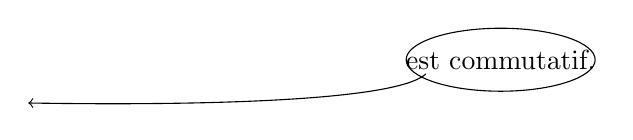
\begin{tikzpicture}[x=1cm,y=1cm]\handwritten{\draw (0,0) ellipse (1.2 and .4);\draw[->] (-.95,-.18) .. controls (-1.45,-.65) and (-5.8,-.55) .. (-6,-.55);}\node at (0,0) {est commutatif.};\end{tikzpicture}}}

$2^\circ)$ si $\handwritten{\varepsilon}:S\handwritten{\to}G$ est la section unité de $G$, le diagramme
\diagram{\begin{tikzcd}[ampersand replacement=\&]
S\handwritten{\times}_S\handwritten{\mathbb{V}}(\handwritten{\mathcal{E}})
 \arrow[rr,"\handwritten{\varepsilon\times}\operatorname{id}_{\handwritten{\mathbb{V}(\mathcal{E})}}"]
\& \& G\handwritten{\times}_S\handwritten{\mathbb{V}}(\handwritten{\mathcal{E}})\arrow[dl,"\handwritten{\theta}"]\\
\& \handwritten{\mathbb{V}}(\handwritten{\mathcal{E}})\arrow[ul,"\handwritten{\sim}"] \&
\end{tikzcd}}
\inserted{\figure{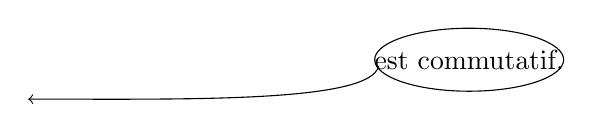
\begin{tikzpicture}[x=1cm,y=1cm]\handwritten{\draw (0,0) ellipse (1.2 and .4);\draw[->] (-1.15,-.08) .. controls (-1.25,-.55) and (-3.6,-.5) .. (-5.6,-.5);}\node at (0,0) {est commutatif.};\end{tikzpicture}}}

Il revient\inserted{\handwritten{alors}} au même de dire que le morphisme $\handwritten{\rho}:\inserted{\handwritten{\mathcal{E}\longrightarrow}}\handwritten{\mathcal{A}}(G)\handwritten{\otimes}_{\handwritten{\mathcal{O}}_{\mathbb{S}}}\handwritten{\mathcal{E}}$ déduit de $\handwritten{\theta}$ vérifie les deux axiomes suivants :
\margin{\handwritten{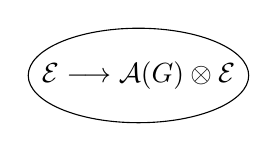
\begin{tikzpicture}
\draw (0,0) ellipse (1.4 and .6);
\node at (0,0) {$\mathcal{E}\longrightarrow\mathcal{A}(G)\otimes\mathcal{E}$};
\end{tikzpicture}}}

(CM1) Si $\handwritten{\Delta}:\handwritten{\mathcal{A}\longrightarrow\mathcal{A}\otimes\mathcal{A}}=\handwritten{\mathcal{A}}(G\handwritten{\times}_S G)$ est l'homomorphisme $\handwritten{\mathcal{A}(\theta)}$, le diagramme
\diagram{\handwritten{\begin{tikzcd}[ampersand replacement=\&]
\mathcal{A}\otimes\mathcal{A}\otimes\mathcal{A}
\& \mathcal{A}\otimes\mathcal{E}\arrow[l,"\operatorname{id}_{\mathcal{A}}\otimes\rho"']\\
\mathcal{A}\otimes\mathcal{E}\arrow[u,"\Delta\otimes\operatorname{id}_{\mathcal{E}}"]
\& \mathcal{A}\arrow[u,"\rho"']\arrow[l,"\rho"]
\end{tikzcd}}}
\inserted{\figure{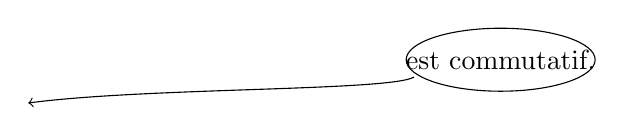
\begin{tikzpicture}[x=1cm,y=1cm]\handwritten{\draw (0,0) ellipse (1.2 and .4);\draw[->] (-1.1,-.22) .. controls (-1.4,-.4) and (-4.5,-.35) .. (-6,-.55);}\node at (0,0) {est commutatif.};\end{tikzpicture}}}

(CM2) Si $\handwritten{\eta}:\handwritten{\mathcal{A}\to\mathcal{O}}_S$ est l'homomorphisme $\handwritten{\mathcal{A}(\varepsilon)}$, le diagramme
\diagram{\handwritten{\begin{tikzcd}[ampersand replacement=\&]
\mathcal{O}_S\otimes\mathcal{E}
\& \& \mathcal{A}\otimes\mathcal{E}\arrow[ll,"\eta\otimes\operatorname{id}_{\mathcal{E}}"']\\
\& \mathcal{E}\arrow[ul,"\sim"]\arrow[ur,"\rho"']\&
\end{tikzcd}}}
\inserted{\figure{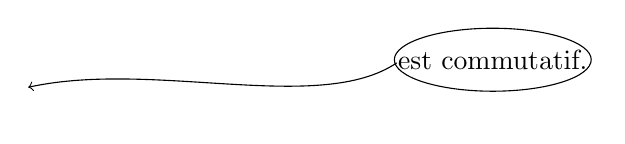
\begin{tikzpicture}[x=1cm,y=1cm]\handwritten{\draw (0,0) ellipse (1.25 and .4);\draw[->] (-1.22,-.04) .. controls (-2.2,-.7) and (-4.3,.0) .. (-5.9,-.35);}\node at (0,0) {est commutatif.};\end{tikzpicture}}}

Il revient au même de dire que le morphisme $\handwritten{\theta}_{\mathrm{af}}:G_{\mathrm{af}}\handwritten{\times}_S\handwritten{\mathbb{V}}(\handwritten{\mathcal{E}})\handwritten{\longrightarrow\mathbb{V}}(\handwritten{\mathcal{E}})$ correspondant à $\handwritten{\rho}$ définit une opération de $G_{\mathrm{af}}$ sur $\handwritten{\mathcal{E}}$ \deleted{\handwritten{\unsure{(Exp. I)}}} \inserted{\handwritten{(\unsure{compar|comparer} I \unsure{4|9}.2)}}.

Par conséquent, il y a correspondance biunivoque entre opérations de $G$ sur $\handwritten{\mathcal{E}}$ et opérations de $G_{\mathrm{af}}$ sur $\handwritten{\mathcal{E}}$.

\uline{\handwritten{L}emme} 11.7.- Soient $G$ un $S$-groupe quasi-compact et quasi-séparé sur $S$\handwritten{,}\inserted{\handwritten{plat et}} tel que $\handwritten{\mathcal{A}}(G)$ soit
% archive sheet number: 45
